\documentclass[tikz,border=5pt]{standalone}
\usepackage{tikz}
\usetikzlibrary{calc}
\definecolor{nebula}{HTML}{6366F1}
\definecolor{spark}{HTML}{14B8A6}
\definecolor{sun}{HTML}{F59E0B}
\definecolor{ink}{HTML}{334155}
\begin{document}
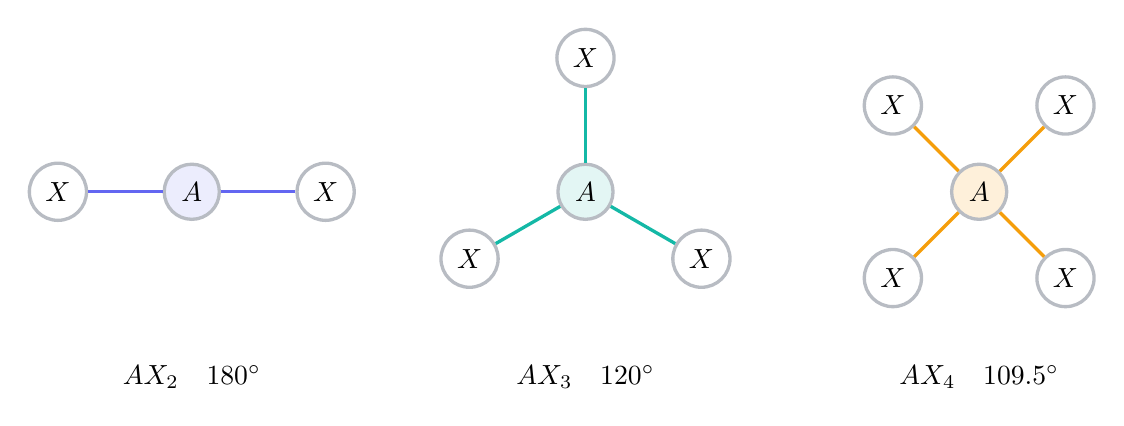
\begin{tikzpicture}[font=\sffamily]
  \tikzset{atom/.style={circle,draw=ink!35,very thick,fill=white,minimum size=7mm}}
  \node[atom,fill=nebula!12] (a2) at (0,0) {$A$};
  \node[atom] (x21) at (-1.7,0) {$X$}; \node[atom] (x22) at (1.7,0) {$X$};
  \draw[very thick,nebula] (x21)--(a2)--(x22);
  \node at (0,-2.35) {$AX_2\quad 180^\circ$};
  \node[atom,fill=spark!12] (a3) at (5,0) {$A$};
  \foreach \p/\n in {90/x31,210/x32,330/x33}{\node[atom] (\n) at ($(a3)+(\p:1.7)$) {$X$}; \draw[very thick,spark] (a3)--(\n);}
  \node at (5,-2.35) {$AX_3\quad 120^\circ$};
  \node[atom,fill=sun!15] (a4) at (10,0) {$A$};
  \foreach \p/\n in {45/x41,135/x42,225/x43,315/x44}{\node[atom] (\n) at ($(a4)+(\p:1.55)$) {$X$}; \draw[very thick,sun] (a4)--(\n);}
  \node at (10,-2.35) {$AX_4\quad 109.5^\circ$};
\end{tikzpicture}
\end{document}
